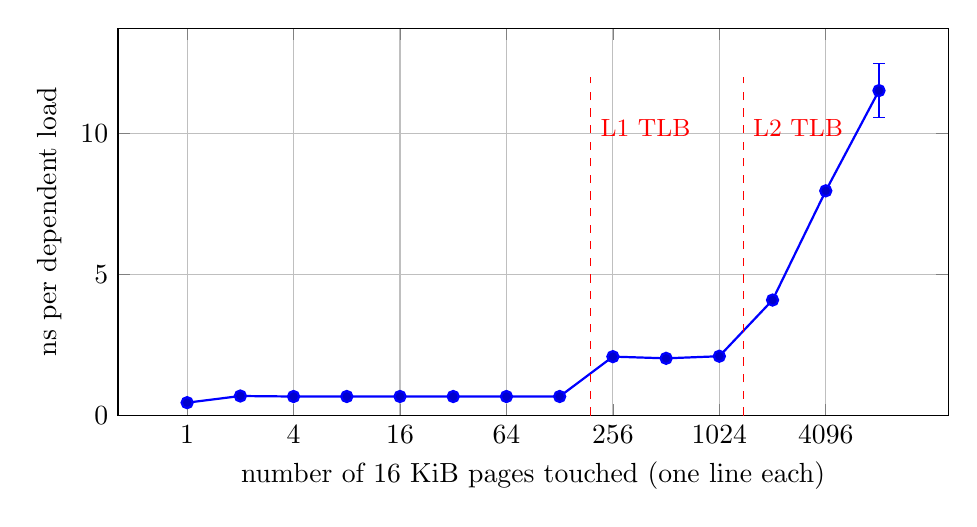
\begin{tikzpicture}
\begin{axis}[width=\textwidth, height=6.5cm, xmode=log, log basis x=2, xlabel={number of 16 KiB pages touched (one line each)}, ylabel={ns per dependent load}, grid=major, ymin=0, xtick={1,4,16,64,256,1024,4096}, xticklabels={1,4,16,64,256,1024,4096}]
\addplot+[mark=*, thick, error bars/.cd, y dir=both, y explicit] coordinates {(1,0.455) +- (0,0.059) (2,0.691) +- (0,0.040) (4,0.673) +- (0,0.000) (8,0.674) +- (0,0.000) (16,0.674) +- (0,0.001) (32,0.673) +- (0,0.000) (64,0.673) +- (0,0.000) (128,0.674) +- (0,0.000) (256,2.086) +- (0,0.040) (512,2.026) +- (0,0.002) (1024,2.100) +- (0,0.049) (2048,4.091) +- (0,0.015) (4096,7.961) +- (0,0.006) (8192,11.513) +- (0,0.962)};
\draw[dashed, red] (axis cs:192,0) -- (axis cs:192,12) node[pos=0.85, right, font=\small] {L1 TLB};
\draw[dashed, red] (axis cs:1400,0) -- (axis cs:1400,12) node[pos=0.85, right, font=\small] {L2 TLB};
\end{axis}
\end{tikzpicture}